%%
%% 中文期刊投稿版（通用格式，可按目标期刊模板调整）
%% 编译方式：xelatex → bibtex → xelatex ×2（Overleaf 上编译器选 XeLaTeX）
%%
% fontset=fandol 在 Overleaf（Linux）与本机均可用
\documentclass[zihao=5,a4paper,linespread=1.3,fontset=fandol]{ctexart}

\usepackage{amsmath}
\usepackage{amssymb}
\usepackage{booktabs}
\usepackage{xcolor}
\usepackage{multirow}
\usepackage{graphicx}
\usepackage{enumitem}
\usepackage[a4paper,top=2.5cm,bottom=2.5cm,left=2.5cm,right=2.5cm]{geometry}
% 部分版本的 gbt7714 在旧式选项分支里残留了调试命令 \foo，此行防止其报错
\providecommand{\foo}{}
\usepackage[super,square,sort&compress]{gbt7714}
\usepackage{hyperref}
\hypersetup{hidelinks}

% --- 浮动体参数 ---
\setcounter{topnumber}{3}
\setcounter{bottomnumber}{2}
\setcounter{totalnumber}{5}
\renewcommand{\topfraction}{0.85}
\renewcommand{\bottomfraction}{0.70}
\renewcommand{\textfraction}{0.15}
\renewcommand{\floatpagefraction}{0.70}

\widowpenalty=10000
\clubpenalty=10000

% ── 记号 ─────────────────────────────────────────────────
\newcommand{\setpoint}{H^*}
\newcommand{\energy}{E}
\newcommand{\drive}{d}
\newcommand{\reward}{r}
\newcommand{\hace}{\textsc{Hace}}

\title{\heiti HACE：以稳态辅助奖励应对序列强化学习中的\\生存可行性失效}
% TODO: 请核实并替换作者中文姓名——“孔××”“桂××”“宋××”为占位符
% （Gui、Song 的姓氏汉字系按常见拼音推断，请务必确认）
\author{孔××，桂××，Ruth Ukubay，宋××\\[0.3em]
{\zihao{-5}（布朗大学~计算机科学系，美国~罗得岛州~普罗维登斯~02912）}\\[0.2em]
{\zihao{-5}\texttt{ziyu\_kong@brown.edu}}}
\date{}

\begin{document}
\maketitle

% ===========================================================================
\begin{abstract}
\noindent{\heiti 摘\quad 要：}持续强化学习（continual reinforcement learning，CRL）研究长期以来几乎完全聚焦于\emph{灾难性遗忘}——神经网络在适应新任务时丧失既有技能的倾向。在智能体需要管理共享生理资源的具身场景中，本文识别出一种与之互补的失效模式：\textbf{生存可行性失效}（viability failure），即智能体在获得学习新任务的机会之前就耗尽内部资源而死亡。弹性权重巩固（EWC）、经验回放（ER）等既有持续强化学习技术作用于参数保持或数据复用而非资源状态管理，因此无法直接应对生存可行性失效。本文提出 \hace{}（Homeostatic Auxiliary for Continual Environments，面向持续环境的稳态辅助奖励）——一种基于稳态驱力降低的任务不变辅助奖励，无需任务定制设计即可激励智能体进行能量管理。在包含 9 种智能体变体的 10 任务资源继承基准以及补充的 5 任务“重置对比继承”析因研究中，\hace{} 智能体的任务边界可解性约为非稳态基线的 3 倍，任务切换时保留的能量约为后者的 3--5 倍，而非稳态基线在本文的生存可行性指标上并未优于无保护基线。将 \hace{} 与 EWC 结合可同时改善生存可行性与知识保持，表明在具身持续强化学习中，维持生存与缓解遗忘是部分可分离的两个问题维度。

\vspace{0.5em}
\noindent{\heiti 关键词：}持续强化学习；灾难性遗忘；生存可行性；稳态强化学习；辅助奖励；具身智能体

\vspace{0.5em}
\noindent{\heiti 中图分类号：}TP181 \qquad {\heiti 文献标识码：}A
\end{abstract}

\vspace{1em}
\begin{center}
{\bfseries HACE: Addressing Viability Failure in Sequential Reinforcement Learning\\ with Homeostatic Auxiliary Rewards}\\[0.5em]
{KONG Ziyu, GUI Shihang, Ruth Ukubay, SONG Meiyi}\\[0.3em]
{\zihao{-5}(Department of Computer Science, Brown University, Providence, RI 02912, USA)}
\end{center}

\vspace{0.5em}
\noindent{\bfseries Abstract:} Continual reinforcement learning (CRL) research has focused almost exclusively on \emph{catastrophic forgetting}---the tendency for neural networks to lose old skills when adapting to new tasks. In embodied settings where agents manage shared physiological resources, we identify a complementary failure mode: \emph{viability failure}, wherein agents deplete internal resources and die before they can learn a new task. Established CRL techniques such as Elastic Weight Consolidation (EWC) and Experience Replay (ER) do not directly address viability failure, because they operate on parameter retention or data reuse rather than resource-state management. We propose HACE (Homeostatic Auxiliary for Continual Environments), a task-invariant auxiliary reward based on homeostatic drive reduction that incentivizes energy management without task-specific engineering. On a 10-task carryover benchmark with 9 agent variants, supplemented by a 5-task reset-vs-carryover factorial study, HACE agents achieve approximately 3$\times$ higher boundary solvability and retain roughly 3--5$\times$ more energy at task transitions than non-homeostatic baselines, which do not improve over unprotected baselines on our viability metrics. Combining HACE with EWC improves both viability and retention, suggesting that viability maintenance and forgetting mitigation are partially separable axes in embodied CRL.

\vspace{0.5em}
\noindent{\bfseries Key words:} continual reinforcement learning; catastrophic forgetting; viability; homeostatic reinforcement learning; auxiliary reward; embodied agents

% ===========================================================================
\section{引言}
\label{sec:intro}

部署于持续学习场景中的强化学习智能体必须在不丧失既有能力的前提下适应不断变化的目标。持续强化学习（CRL）领域的主流研究范式几乎完全将这一挑战归结为\emph{灾难性遗忘}：参数在新任务训练过程中覆盖旧知识的倾向\cite{Parisi2019,kirkpatrick2017,continualworld2021}。围绕这一问题已发展出丰富的方法工具箱——弹性权重巩固（EWC\cite{kirkpatrick2017}）、经验回放（ER\cite{rolnick2019}）、渐进式网络架构\cite{rusu2016}——它们的评价标准都是旧任务性能在新任务训练后是否退化。

我们认为，这种对遗忘的聚焦掩盖了\emph{具身}序列场景中另一个同样关键的失效模式：\textbf{生存可行性失效}（viability failure）。当环境施加共享的生理约束——例如随每步动作消耗的内部能量变量——时，任务切换可能是致命的。以极低剩余能量完成任务 $T_i$ 的智能体，抵达任务 $T_{i+1}$ 时已没有足够资源存活到学会新任务。无论怎样的权重正则化或经验重放，都救不了一个在新任务前三步就死亡的智能体。

考虑一个具体例子。在 \textsc{Conservation}（高单步能耗，必须节约）上训练的智能体切换到 \textsc{Sprint}（时间限制极短，必须求快）。在继承边界条件下——能量跨任务保留——智能体以危险的低能量抵达 \textsc{Sprint}，且没有时间探索，随即死亡。EWC 完美保住了 \textsc{Conservation} 的权重，但如果智能体无法存活，这些权重毫无用处。

本文有三项贡献。第一，我们正式将\textbf{生存可行性失效}识别为具身持续强化学习中与灾难性遗忘不同的独立失效模式，并证明传统 CRL 方法并不直接针对它（第~\ref{sec:method}~节）。第二，我们提出 \textbf{\hace{}}——一种基于稳态驱力降低的任务不变辅助奖励，无需任务定制设计即可在所有任务中激励能量管理。第三，我们设计了一个包含 9 种智能体变体与精心编排任务序列的 \textbf{10 任务序列网格世界基准}，支持对两种失效模式的系统研究（第~\ref{sec:setup}~节）。实验（第~\ref{sec:results}~节）表明，\hace{} 能在任务切换中维持生存可行性，而传统 CRL 方法在本文基准的生存指标上没有改善。

% ===========================================================================
\section{相关工作}
\label{sec:related}

\paragraph{持续强化学习。}
EWC\cite{kirkpatrick2017} 通过 Fisher 信息加权的惩罚项约束重要参数；ER\cite{rolnick2019} 在新任务训练中穿插重放旧转移样本；渐进式网络\cite{rusu2016} 冻结旧网络列并逐任务扩充容量。这些方法在 Continual World\cite{continualworld2021} 与 CORA\cite{cora2022} 等基准上得到评测，而这些基准中的回合终止不受资源约束影响。本文指出，这种评测范式并不直接检验生存可行性失效。

\paragraph{稳态强化学习。}
Keramati 与 Gutkin\cite{keramati2014} 将奖励形式化为内部设定点偏差的降低，由此产生风险规避与前瞻性行为。Yoshida\cite{yoshida2018,Yoshida} 将其扩展到深度强化学习并与元强化学习相联系。Konidaris 与 Barto\cite{konidaris2006} 提出了自适应动机系统。然而这些先行工作大多研究单一或缓慢变化的环境，未曾检验稳态目标是否能改善序列任务学习。

\paragraph{迁移与辅助奖励。}
后继特征（successor features）\cite{Barreto}将价值函数分解为可复用的动力学部分与任务特定权重。Tomov 等\cite{Tomov} 观察到人类会跨任务复用策略，且任务描述可以落地到生理状态——\hace{} 正是将这一洞见付诸实现。与好奇心驱动\cite{pathak2017}或像素控制\cite{jaderberg2017}不同，\hace{} 的目标是\emph{维持生存可行性}，而非探索或表征学习。

% ===========================================================================
\section{生存可行性失效与 HACE 方法}
\label{sec:method}

\subsection{序列任务设定}

我们考虑智能体依次学习任务序列 $T_1, \ldots, T_n$，各任务共享动作空间、内部能量变量 $\energy_t \in [0, \energy_{\max}]$（单步消耗 $c_{\text{step}}$），以及终止条件 $\energy_t \leq 0 \implies$ 死亡。任务在网格布局、危险格、食物源、墙体与能量经济设置上互不相同（第~\ref{sec:setup}~节）。在任务边界处，智能体保留网络参数；能量则由\emph{边界模式}决定：\textbf{重置}（reset）将能量重新初始化为各任务默认值，\textbf{继承}（carryover）保留上一任务结束时的剩余能量。继承是生态上更真实的设定，也是生存可行性失效最严重的场景。

\subsection{生存可行性失效}

当智能体在任务 $T_i$ 结束时的期望剩余能量不足以支撑其在 $T_{i+1}$ 中的探索时，就在边界 $T_i \to T_{i+1}$ 处发生生存可行性失效：
\begin{equation}
  \mathbb{E}_{\pi_i}\!\left[\energy_{T_i}^{\text{terminal}}\right]
  \;<\; \energy_{\text{viable}}^{(i+1)}.
\end{equation}
此时智能体在新任务开始的最初几步内死亡，观测到的几乎全是短促的死亡轨迹，得不到关于新任务成功行为的有效信号。这与灾难性遗忘有本质区别：遗忘是\emph{参数层面}的问题（旧权重被覆盖），而生存可行性失效是\emph{轨迹层面}的问题（智能体存活时间不足以学习）。EWC 能完美保留旧权重，却无法迫使智能体节约能量；ER 重放旧转移样本，但这些样本并不必然改善智能体在新任务边界处的资源枯竭状态；L2 正则化约束参数范数，与生存信号毫无关联。因此，这些方法针对的是参数或数据的保持，而生存可行性失效取决于智能体在任务边界处的实际资源状态。

在实验中，我们通过边界可解性对生存可行性阈值进行经验化操作化：即策略从上一任务的终端能量分布出发初始化时，能否完成下一任务。

\subsection{稳态驱力降低}

沿用 Keramati 与 Gutkin\cite{keramati2014} 的框架，我们将内部驱力定义为与稳态设定点 $\setpoint$ 的距离：$\drive_t = |\setpoint - \energy_t|$。\hace{} 辅助奖励即单步驱力降低量：
\begin{equation}
  \reward_t^H \;=\; |\setpoint - \energy_t| \;-\; |\setpoint - \energy_{t+1}|.
  \label{eq:drive}
\end{equation}
当动作使智能体趋近稳态（如低能量时收集食物）时该信号为正，使偏差增大时为负。其函数形式是\emph{任务不变}的：智能体在所有任务中接收相同的驱力降低信号，能量按各任务的能量上限归一化。该信号同时是\emph{稠密}的（逐步反馈）且具有\emph{生物学动机}（对应生物体的驱力降低机制\cite{keramati2014,konidaris2006}）。

完整的 \hace{} 奖励将其与任务特定信号组合：$\reward_t^{\text{HACE}} = \alpha \cdot \reward_t^{\text{task}} + \reward_t^H$，默认 $\alpha = 1.0$ 且 $\setpoint = \energy_{\text{cap}}$。在本基准中，将稳态设定点取为能量上限使 \hace{} 成为一种保守的能量保全信号：智能体因避免以枯竭状态抵达边界而获得奖励，而不仅仅是最大化任务奖励。我们采用这一实例化是因为本文环境的核心风险是能量耗尽致死；其他领域可能需要中间值或自适应的设定点。由于 \hace{} 作用于\emph{奖励层面}而 EWC/ER 作用于\emph{权重/数据层面}，二者天然互补：智能体~I（\hace{}+EWC）将两者结合，同时应对生存与遗忘。

% ===========================================================================
\section{实验设置}
\label{sec:setup}

\subsection{任务基准}

我们设计了包含 12 个结构各异的网格世界任务的任务目录，并从中实例化精心编排的 10 任务序列用于序列训练。所有任务共享相同的能量动力学，但在空间布局、危险格、食物摆放、墙体、闸门机制、单步消耗与能量容量上各不相同。表~\ref{tab:tasks} 汇总了任务目录。每个任务都是一个 Gymnasium 环境：智能体在离散网格上移动，每步消耗能量，收集食物以恢复能量，躲避危险格，并绕过墙体与闸门机制。回合在成功抵达出口或能量耗尽时终止。

\begin{table}[t]
\centering
\caption{任务目录。所有任务共享 4 个移动动作与“能量耗尽即终止”规则。$c_s$：单步消耗；F：食物数量；H：危险格数量。任务名保留英文原名。}
\label{tab:tasks}
\small
\setlength{\tabcolsep}{5pt}
\begin{tabular}{@{}lcccccl@{}}
\toprule
\textbf{任务} & \textbf{网格} & $\energy_0$ & $c_s$ &
\textbf{F} & \textbf{H} & \textbf{核心挑战} \\
\midrule
Reach          & 5 & 15 & 1 & 1 & 0 & 导航 \\
Recharge       & 5 &  8 & 1 & 1 & 0 & 必须进食才能存活 \\
Hazard Cross   & 5 & 12 & 1 & 1 & 2 & 躲避危险 \\
Detour         & 5 &  9 & 1 & 1 & 2 & 进食 + 躲避 \\
Wall Maze      & 6 & 14 & 1 & 1 & 0 & 空间规划 \\
Dual Food      & 6 & 10 & 1 & 2 & 1 & 稀缺下的决策 \\
Haz.~Gauntlet  & 6 & 14 & 1 & 1 & 4 & 密集危险 \\
Conservation   & 5 & 20 & 2 & 1 & 1 & 高单步消耗 \\
Endurance      & 7 & 16 & 1 & 1 & 2 & 长路径 \\
Collect Exit   & 6 & 14 & 1 & 1 & 2 & 闸门机制 \\
Sprint         & 5 & 14 & 1 & 1 & 0 & 极短时间限制 \\
Gaunt.~Refuel  & 7 & 16 & 1 & 2 & 4 & 全技能综合 \\
\bottomrule
\end{tabular}
\end{table}

我们定义了三种精心编排的 10 任务排序：\textbf{$\alpha$（能量迁移）}，能量管理技能逐级累积；\textbf{$\beta$（安全迁移）}，先学习躲避技能；\textbf{$\gamma$（干扰）}，刻意安排策略相互冲突的任务（如 Conservation $\to$ Sprint）。完整排序见附录~\ref{app:sequences}。

\subsection{智能体目录}

我们比较 9 种智能体变体（表~\ref{tab:agents}），系统地改变奖励信号、能量观测、CRL 方法与训练模式。所有变体共享相同的 DQN 架构（2 层 MLP，128 隐藏单元，$\varepsilon$-贪心；详见附录~\ref{app:hyperparams} 与~\ref{app:obs}）。

\begin{table}[t]
\centering
\caption{智能体目录。TR：任务奖励；EO：能量观测；HR：稳态奖励；Seq：序列训练（参数继承）。}
\label{tab:agents}
\small
\setlength{\tabcolsep}{4.5pt}
\begin{tabular}{@{}llccccc@{}}
\toprule
\textbf{编号} & \textbf{智能体} & \textbf{TR} & \textbf{EO} &
\textbf{HR} & \textbf{CRL} & \textbf{Seq} \\
\midrule
A & 仅任务奖励          & \checkmark & --  & --  & --     & \checkmark \\
B & 能量感知       & \checkmark & \checkmark & --  & --     & \checkmark \\
C & \textbf{HACE}      & \checkmark & \checkmark & \checkmark & --     & \checkmark \\
D & 纯稳态   & --  & \checkmark & \checkmark & --     & \checkmark \\
E & 任务先知        & \checkmark & \checkmark & --  & --     & -- \\
F & EWC                & \checkmark & \checkmark & --  & EWC    & \checkmark \\
G & L2                 & \checkmark & \checkmark & --  & L2     & \checkmark \\
H & 经验回放        & \checkmark & \checkmark & --  & ER     & \checkmark \\
I & \textbf{HACE+EWC}  & \checkmark & \checkmark & \checkmark & EWC    & \checkmark \\
\bottomrule
\end{tabular}
\end{table}

\subsection{评价指标}

我们从以下维度评价智能体：\textbf{当前任务成功率}（评估回合中抵达出口的比例）、\textbf{阶段末评估矩阵} $R_{i,j}$（训练完 $T_i$ 后在任务 $T_j$ 上的成功率）、\textbf{边界可解性}（当前策略能否从其在 $T_i$ 的实际终端能量出发解决 $T_{i+1}$）、任务边界处的\textbf{平均终端能量}，以及标准\textbf{遗忘度} $F_j = \max_{i \geq j} R_{i,j} - R_{n,j}$。

\subsection{实验协议}

所有实验在继承边界模式（最具挑战性的设定）下使用 $\alpha$ 序列，每任务 600 个回合，每 50 个训练回合进行 40 个评估回合，每种智能体 10 个随机种子。尽管基准定义了三种排序，本研究聚焦于主排序 $\alpha$；其余排序用于记录基准设计并支持后续工作。我们报告均值与标准差。第~\ref{sec:factorial}~节另行比较重置与继承两种模式。

% ===========================================================================
\section{实验结果}
\label{sec:results}

\subsection{9 智能体全套实验（10 任务 $\alpha$ 序列，继承模式）}
\label{sec:full_suite}

图~\ref{fig:learning} 展示了 9 种智能体在 10 任务序列上的学习曲线。为减少视觉干扰，我们突出显示四个主要智能体——仅任务奖励（A）、\hace{}（C）、EWC（F）与 \hace{}+EWC（I）——其余五个以背景线呈现。

\begin{figure*}[t]
  \centering
  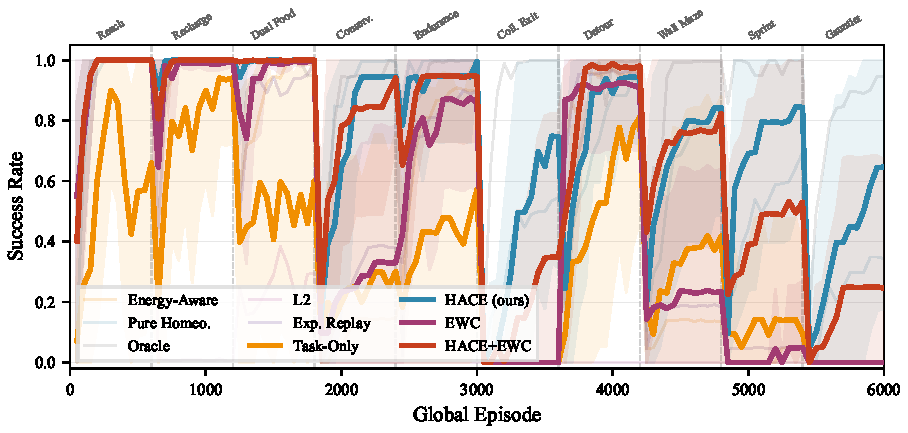
\includegraphics[width=\textwidth]{figures/fig_learning_curves.pdf}
  \caption{10 任务 $\alpha$ 序列（继承模式）下的当前任务成功率（图中文字为英文）。虚线标记任务边界。\hace{}（青色）与 \hace{}+EWC（朱红色）在任务切换处持续恢复，而仅任务奖励（琥珀色）与 EWC（紫红色）在后期任务上崩溃。背景线为其余智能体。10 个种子的均值 $\pm\,1\sigma$。}
  \label{fig:learning}
\end{figure*}

学习曲线中可见几个模式。第一，传统 CRL 方法（EWC、L2、ER）在序列后半段相对无保护的仅任务奖励基线没有任何生存优势。在任务 7--10（Detour 至 Gauntlet Refuel）上，缺乏稳态奖励的智能体在最难的后期任务上成功率常常趋近于零。第二，\hace{} 智能体（C 与 I）在任务边界处的初始下跌后持续恢复，表明稳态奖励提供了持久的生存信号，支撑其在新任务中的探索。第三，\hace{}+EWC（I）在全序列上表现最为稳定，兼具 \hace{} 的生存优势与 EWC 对早期任务的权重保护。

图~\ref{fig:boundary} 直接量化了生存机制。子图~(a) 给出平均边界可解性：\hace{} 与 \hace{}+EWC 的边界可解性约为非稳态基线的 3 倍。这支持了生存可行性失效是主要瓶颈的判断——仅保护权重的 CRL 方法并不能提高智能体在下一任务中的存活能力。子图~(b) 揭示了根本原因：\hace{} 智能体在任务边界处保留的能量是其他智能体的 3--5 倍（11.2 与 9.1，其余智能体为 2--4），直接支撑了持续探索。

\begin{figure}[t]
  \centering
  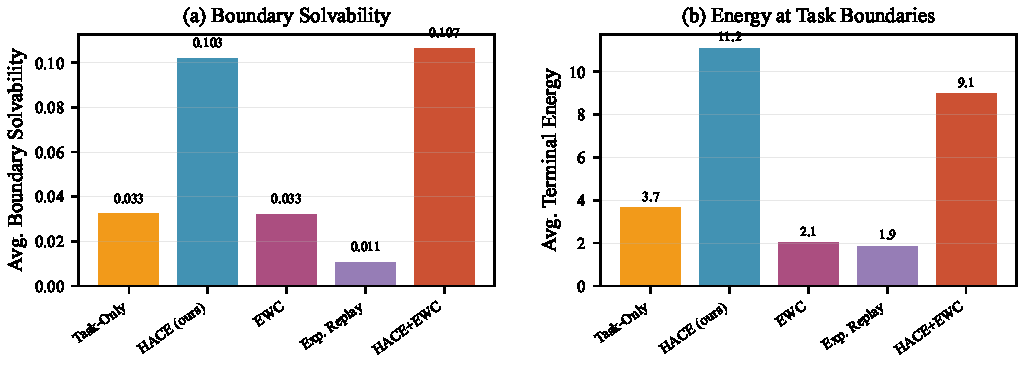
\includegraphics[width=\columnwidth]{figures/fig_boundary_energy.pdf}
  \caption{(a) 9 次任务切换的平均边界可解性。(b) 任务边界处的平均终端能量。\hace{} 变体保留的能量是所有 CRL 基线的 3--5 倍，直接带来更高的边界可解性（图中文字为英文）。}
  \label{fig:boundary}
\end{figure}

图~\ref{fig:heatmap} 给出序列末的成功率矩阵。热力图概括了序列结束时的对比：仅任务奖励（A）在完成全序列后对全部 10 个任务的保持成功率几乎为零，而 \hace{}+EWC（I）在最难的综合任务 Gauntlet Refuel 上维持 $>$0.25 的成功率，并取得所有任务上最高的平均成功率（0.335）。即使是 EWC（F）与 ER（H），尽管对早期任务性能有一定保护（Reach：0.40--0.53），在最终任务上的成功率也接近零。单独的 \hace{}（C）在 Gauntlet Refuel 上取得非先知智能体中的最高成功率（$>$0.60）——该任务要求导航、食物收集、危险躲避与高效能量利用全部四项技能。

\begin{figure}[!htb]
  \centering
  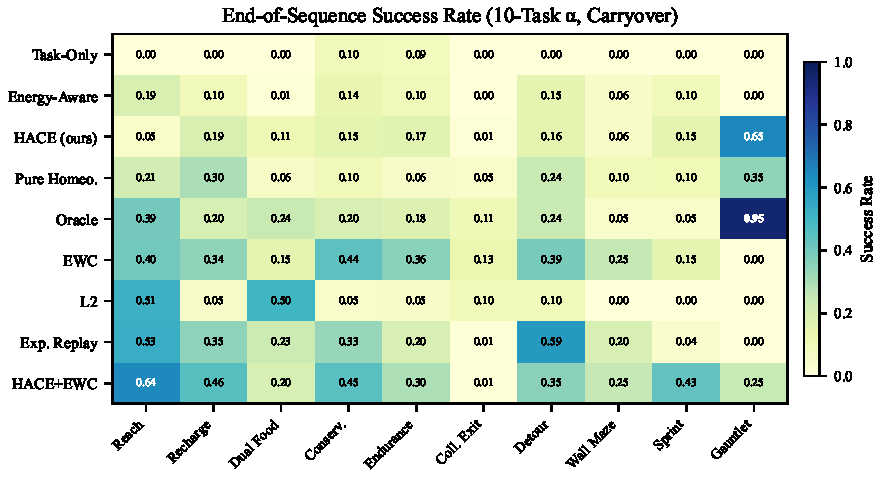
\includegraphics[width=\columnwidth]{figures/fig_performance_heatmap.pdf}
  \caption{10 任务 $\alpha$ 序列（继承模式）序列末成功率（智能体 $\times$ 任务）（图中文字为英文）。颜色越深成功率越高。\hace{}+EWC（底行）平均性能最高；\hace{}（C）在 Gauntlet Refuel 上取得最强的非先知性能。}
  \label{fig:heatmap}
\end{figure}

\subsection{重置对比继承：隔离生存可行性失效}
\label{sec:factorial}

为确认继承模式下的性能崩溃源于生存可行性失效而非遗忘，我们在 5 任务先导序列上开展了 $3 \times 2$ 析因实验（3 种奖励机制 $\times$ 2 种边界模式），每种条件 10 个随机种子。

\begin{figure}[!htb]
  \centering
  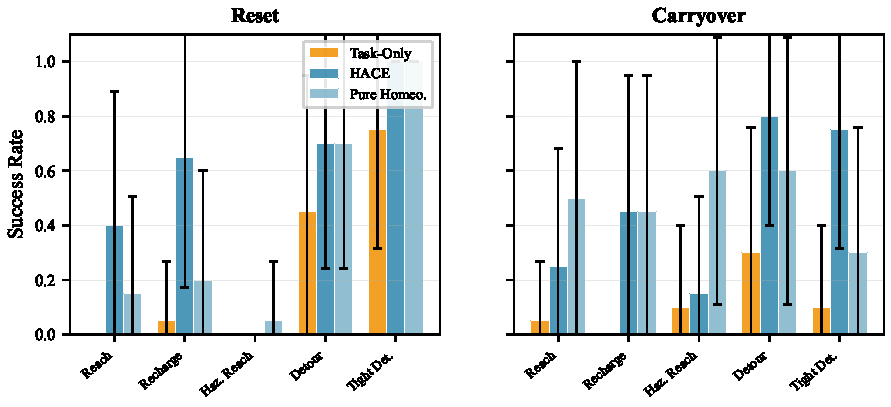
\includegraphics[width=\columnwidth]{figures/fig_viability_collapse.pdf}
  \caption{重置（左）与继承（右）模式下的最终评估（图中文字为英文）。重置模式下所有智能体表现相当；继承模式下仅任务奖励（琥珀色）退化而 \hace{}（青色）保持性能。这一差异支持生存可行性失效是主要解释：当边界能量被重置时，同样的任务序列与学习设置下性能得以恢复。}
  \label{fig:collapse}
\end{figure}

图~\ref{fig:collapse} 提供了直接证据。重置模式下，三种奖励机制表现相当：仅任务奖励在 Detour 上达到 0.45--0.75 的成功率。继承模式下，仅任务奖励跌至 0.30，而 \hace{} 保持 0.80。关键在于，任务定义、网络架构与训练协议完全固定，唯一的操纵变量是能量在任务边界处重置还是继承。这支持了如下解释：驱动所观察到崩溃的是资源状态的跨任务继承，而不仅仅是遗忘。稳态智能体保持更高的终端能量（序列末 2.95，仅任务奖励为 0.35），直接转化为后续任务中的存活。

% ===========================================================================
\section{讨论与结论}
\label{sec:discussion}

本文的结果确立了三项对持续强化学习研究议程具有启示意义的发现。

\paragraph{生存可行性失效是一种独立的、被忽视的失效模式。}
重置对比继承实验（第~\ref{sec:factorial}~节）表明，继承条件下的性能崩溃并非灾难性遗忘——在相同任务序列与训练设置下，只要重置边界能量，性能便得以恢复。9 智能体全套实验显示，既有 CRL 方法（EWC、L2、ER）在某些情形下改善知识保持，但不改善边界生存指标。这说明标准 CRL 基准往往没有建模跨任务边界继承的共享内部资源，可能忽视了具身场景中的一种重要失效模式。

\paragraph{HACE 简单、有效，且与 CRL 方法互补。}
\hace{} 辅助奖励（式~\ref{eq:drive}）只需对任意强化学习训练循环做一行修改。它不需要为各任务手工设计奖励，不需要架构改动，只有少量透明的奖励超参数——却带来约 3 倍的边界可解性提升，并使智能体 C 在 Gauntlet Refuel 上取得最强的非先知性能（成功率 0.65）。智能体~I（\hace{}+EWC）兼得两者之长：\hace{} 级别的生存能力加上 EWC 对早期任务的保持，取得最高的总体平均成功率（0.335）。这种互补性提示了具身持续强化学习问题的一种原则性分解：\emph{活下去}（奖励层面）与\emph{记住怎么做}（权重层面）是部分可分离的两个维度，各自受益于独立的解决方案。

\paragraph{局限性与未来工作。}
本文基准采用向量观测的表格型网格世界；确认结论的普适性需要扩展到视觉输入与更丰富的三维环境。所有结果均基于 DQN，用策略梯度或 Transformer 架构复现将进一步验证发现。我们只建模了单一资源（能量），而真实智能体需要管理多个耦合的驱力。最后，我们固定 $\setpoint = \energy_{\text{cap}}$；逐任务学习或自适应设定点仍未探索。尽管基准的简单性限制了对普适性的断言，这些结果表明生存可行性失效是研究具身持续强化学习的一个有用视角，而 \hace{} 的简单性使其易于在其他具有共享资源约束的具身序列强化学习场景中检验。

\bibliography{refs}

% ===========================================================================
\clearpage
\appendix

\section{超参数}
\label{app:hyperparams}

表~\ref{tab:hyperparams} 列出所有智能体共享的训练超参数，以及智能体特定参数（EWC $\lambda$、ER 蓄水池大小等）。

\begin{table}[h]
\centering
\caption{训练超参数。}
\begin{tabular}{@{}ll@{}}
\toprule
\textbf{参数} & \textbf{取值} \\
\midrule
网络架构 & 2 层 MLP，128 隐藏单元 \\
优化器 & Adam \\
学习率 & $5 \times 10^{-4}$ \\
折扣因子 $\gamma$ & 0.99 \\
批大小 & 64 \\
回放缓冲区 & 20\,000 条转移 \\
目标网络更新 & 每 25 回合 \\
$\varepsilon$-贪心 & 1.0 $\to$ 0.05（300 回合内） \\
每任务回合数 & 600 \\
评估 & 每 50 训练回合评估 40 回合 \\
\midrule
EWC $\lambda$（F、I） & 400.0 \\
EWC Fisher 采样数 & 1\,000 \\
L2 $\lambda$（G） & 100.0 \\
ER 蓄水池（H） & 5\,000 条转移，比例 0.5 \\
\hace{} 设定点 & 各任务的 $\energy_{\text{cap}}$ \\
\hace{} 系数 & 1.0 \\
任务奖励系数 $\alpha$ & 1.0 \\
\bottomrule
\end{tabular}
\label{tab:hyperparams}
\end{table}

\section{任务序列定义}
\label{app:sequences}

表~\ref{tab:sequences} 列出实验使用的三种 10 任务排序。$\alpha$ 序列是正文所有实验采用的主排序；$\beta$ 与 $\gamma$ 保留用于未来的跨序列泛化分析。

\begin{table}[h]
\centering
\caption{完整的 10 任务序列排序。}
\label{tab:sequences}
\begin{tabular}{@{}cp{0.82\textwidth}@{}}
\toprule
\textbf{序列} & \textbf{任务顺序} \\
\midrule
$\alpha$ & Reach $\to$ Recharge $\to$ Dual Food $\to$ Conservation $\to$
           Endurance $\to$ Collect Exit $\to$ Detour $\to$ Wall Maze $\to$
           Sprint $\to$ Gauntlet Refuel \\
\midrule
$\beta$  & Reach $\to$ Hazard Cross $\to$ Haz.~Gauntlet $\to$ Wall Maze $\to$
           Detour $\to$ Recharge $\to$ Sprint $\to$ Conservation $\to$
           Collect Exit $\to$ Gauntlet Refuel \\
\midrule
$\gamma$ & Conservation $\to$ Sprint $\to$ Haz.~Gauntlet $\to$ Reach $\to$
           Endurance $\to$ Dual Food $\to$ Hazard Cross $\to$ Collect Exit $\to$
           Recharge $\to$ Wall Maze \\
\bottomrule
\end{tabular}
\end{table}

\section{预实验：5 任务序列先导研究}
\label{app:pilot}

在部署 9 智能体全套实验之前，我们先以较小规模的先导实验验证核心假设。我们在 5 任务旧版序列 Reach $\to$ Recharge $\to$ Hazard Cross $\to$ Detour $\to$ Sprint 上训练了两种智能体——任务奖励基线（有能量观测但无稳态奖励）与纯稳态基线（与智能体~D 相当），每任务 600 回合，10 个随机种子。

先导实验（图~\ref{fig:pilot}）揭示了一个一致的权衡：任务特定奖励在早期简单任务上学得更快（Reach：200 回合内达到 0.6，稳态智能体需 400 回合），但稳态智能体在需要资源管理与危险躲避的后期任务上追平或超越。Hazard Cross 上的最终保持为 0.90 对 0.70，Detour 上为 0.80 对 0.60。这一初步发现促成了正文的 9 智能体全套实验。

\begin{figure}[h]
  \centering
  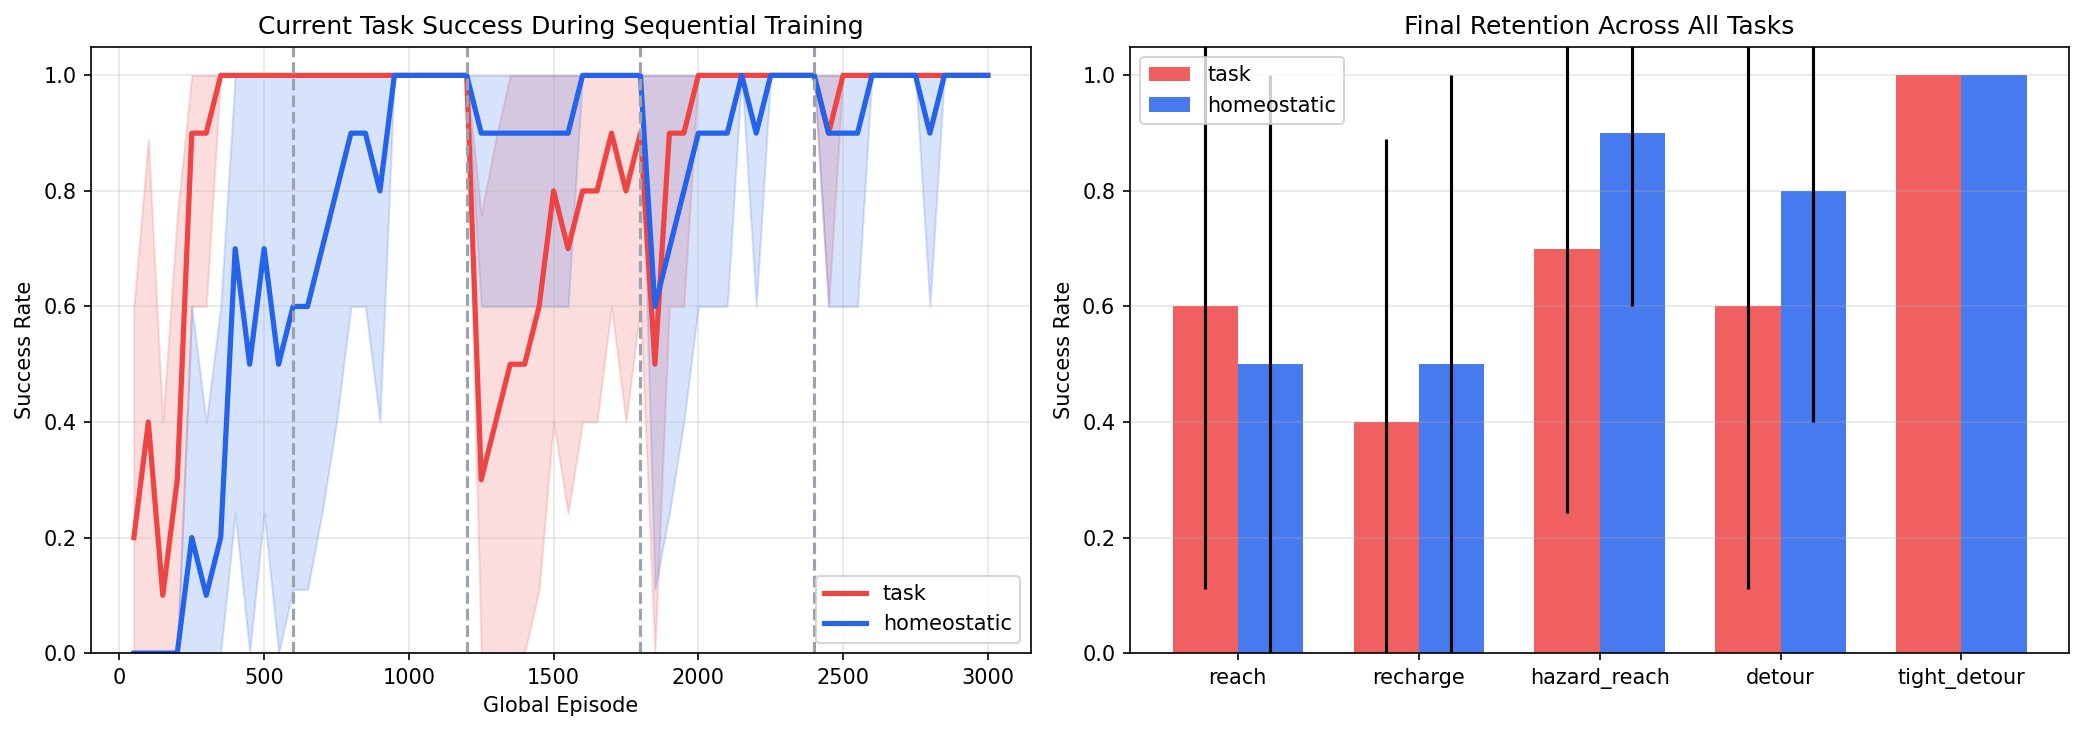
\includegraphics[width=0.85\textwidth]{figures/sequential_pilot.png}
  \caption{5 任务序列先导实验（图中文字为英文）。\emph{左}：序列训练期间的当前任务成功率。任务特定奖励智能体（红色）在早期任务上学得更快；稳态智能体（蓝色）在后期任务上追平或超越。\emph{右}：全部五个任务的最终保持。稳态智能体在依赖资源管理的任务上保持更强（Hazard Cross：0.90 对 0.70；Detour：0.80 对 0.60）。}
  \label{fig:pilot}
\end{figure}

\section{观测空间细节}
\label{app:obs}

所有智能体使用相同的 19 维观测布局（表~\ref{tab:obs}）。对于无能量观测的智能体，能量坐标以哨兵值（$-1$）遮蔽，使输入维度在各智能体间保持一致。观测编码了智能体位置、目标位置、食物与危险格位置，以及——关键地——智能体当前能量水平。所有空间特征按网格尺寸归一化；能量按任务的能量上限归一化。

\begin{table}[h]
\centering
\caption{观测向量布局。所有空间特征归一化到 $[0,1]$。智能体~A 接收遮蔽的能量值（$-1$），以便将奖励信号的作用与观测内容隔离。}
\label{tab:obs}
\small
\begin{tabular}{@{}cll@{}}
\toprule
\textbf{索引} & \textbf{内容} & \textbf{归一化} \\
\midrule
0--1 & 智能体位置（行、列） & $/$（grid\_size $-$ 1） \\
2--3 & 出口位置（行、列） & $/$（grid\_size $-$ 1） \\
4--6 & 食物 1：行、列、可用 & $/$~网格；布尔值 \\
7--9 & 食物 2：行、列、可用 & $/$~网格；布尔值 \\
10   & 能量水平 & $/$~energy\_cap（遮蔽时为 $-1$） \\
11   & 任务索引 & $/$（num\_tasks $-$ 1） \\
12--17 & 危险格位置（至多 3 个） & $/$~网格（缺省为 $-0.25$） \\
18   & 闸门锁定 & 布尔值 \\
\bottomrule
\end{tabular}
\end{table}

\end{document}
